\chapter{Equations with a small parameter}
A small parameter in the differential equation can appear in essentially two ways:  either on the right side or on the left side. In the first case we deal with a small perturbation of the system, which we know a lot about in general and in the second case they are so-called relaxation oscillations. Both cases are discussed in successive sections.

\section{Averaging}
An example of a system from the first group is the known Van der Pole system
$$
\dot{x}=y,\text{ \ }\dot{y}=-x+\varepsilon (1-x^{2})y,
$$
where $\varepsilon$ is our small parameter. This is a special case of a perturbation of the Hamiltonian system with one degree of freedom (with the Hamiltonian function: $H(x,y)=1/2 x^2 + 1/2 y^2$)
\begin{equation}
\label{4.1}
\dot{x} = \frac{\partial H}{\partial y} +\varepsilon P(x,y),\text{ \ \ }\dot{y}%
=-\frac{\partial H}{\partial x} +\varepsilon Q(x,y).
\end{equation}
In applications often appear Hamiltonian systems with many degrees of freedom of the form 
\begin{equation}
\label{4.2}
\dot{q}_{i}= \frac{\partial H}{\partial p_i},\text{ \ \ }\dot{p}_{i}=- \frac{\partial H}{\partial q_i},%
\text{ \ \ \ }i=1,\ldots n,
\end{equation}
where $q_i$ are generalized coordinates, $p_i$ are generalized momenta and the function \linebreak
$H(q_{1}, \ldots, q_{n}, p_{1}, \ldots, p_{n})$ is a \textbf{hamiltonian function}, or \textit{Hamiltonian} (Tasks 4.11 and 4.12). In general, the system \eqref{4.2} can not be solved. However, there is a class of Hamiltonian systems fully solvable.

\begin{definition}\label{def:4.1}
	The system \eqref{4.2} is called \textbf{completely integrable} if there is a system of \textbf{functionally independent} of the first integrals $F_1 = H, F_2,\ldots , F_n$ such that each function $F_j$ is the first integral for other Hamiltonian systems generated by other $F_i$ functions. It is also said that the \textit{functions} $F_j$ \textit{are in involution}, i.e.
	$$ \sum_{i=1}^{n} \frac{\partial F_i}{\partial q_i} \dot{q_i} + \sum_{i=1}^{n} \frac{\partial F_i}{\partial p_i} \dot{p_i} = \sum_{i=1}^{n} \frac{\partial F_i}{\partial q_i} \frac{\partial F_k}{\partial p_i} + \sum_{i=1}^{n} \frac{\partial F_i}{\partial p_i} \left( -\frac{\partial F_k}{\partial q_i}\right) = 0.$$
\end{definition}

Examples of completely integrable systems are the Kepler problem and geodesic flow on the surface of an ellipsoid (see \cite{Ar3}); both have two degrees of freedom.

For systems that satisfy the condition of Definition \ref{def:4.1}, the following statement is made, which we quote without proof (see \cite{Ar3}).

\begin{theorem} \emph{(Liouville-Arnold).}\label{theo:4.4}
	If the common levels $\{F_{1}=c_{1},\ldots ,$ $F_{n}=c_{n}\}$ of a completely integrable Hamiltonian system are compact and smooth, these are the $\mathbb{T}^n$ torus.
	
	In addition, in the neighborhood of a given torus there is a system of coordinates $\left( I_{1},\ldots ,I_{n},\varphi _{1},\ldots ,\varphi
	_{n}\right) $, the so-called \textbf{action-angle variables}, in which the system \eqref{4.2} takes the following Hamiltonian form 
	\begin{equation}
	\label{4.3}
	\dot{I}_{j}=0,\text{ \ \ }\dot{\varphi}_{j}=\omega _{j}(I)=\partial
	H_{0}/\partial I_{j},\text{ \ \ \ \ }j=1,\ldots ,n,
	\end{equation}
	where $H(q,p)=H_{0}(I_{1},\ldots ,I_{n})$ is the Hamiltonian after the exchange. In general, torus movement $\left\{
	I_{1}=d_{1},\ldots ,I_{n}=d_{n}\right\} $, which are parameterized by angles $\varphi _{j}$ mod $2\pi $, is periodic or quasi-periodic (see Figure \ref{fig:4.1}):
	$$
	\varphi _{j}(t)=\varphi _{j}(0)+\omega _{j}(I)t.
	$$
\end{theorem}

\begin{figure}[!ht]
	\centering
	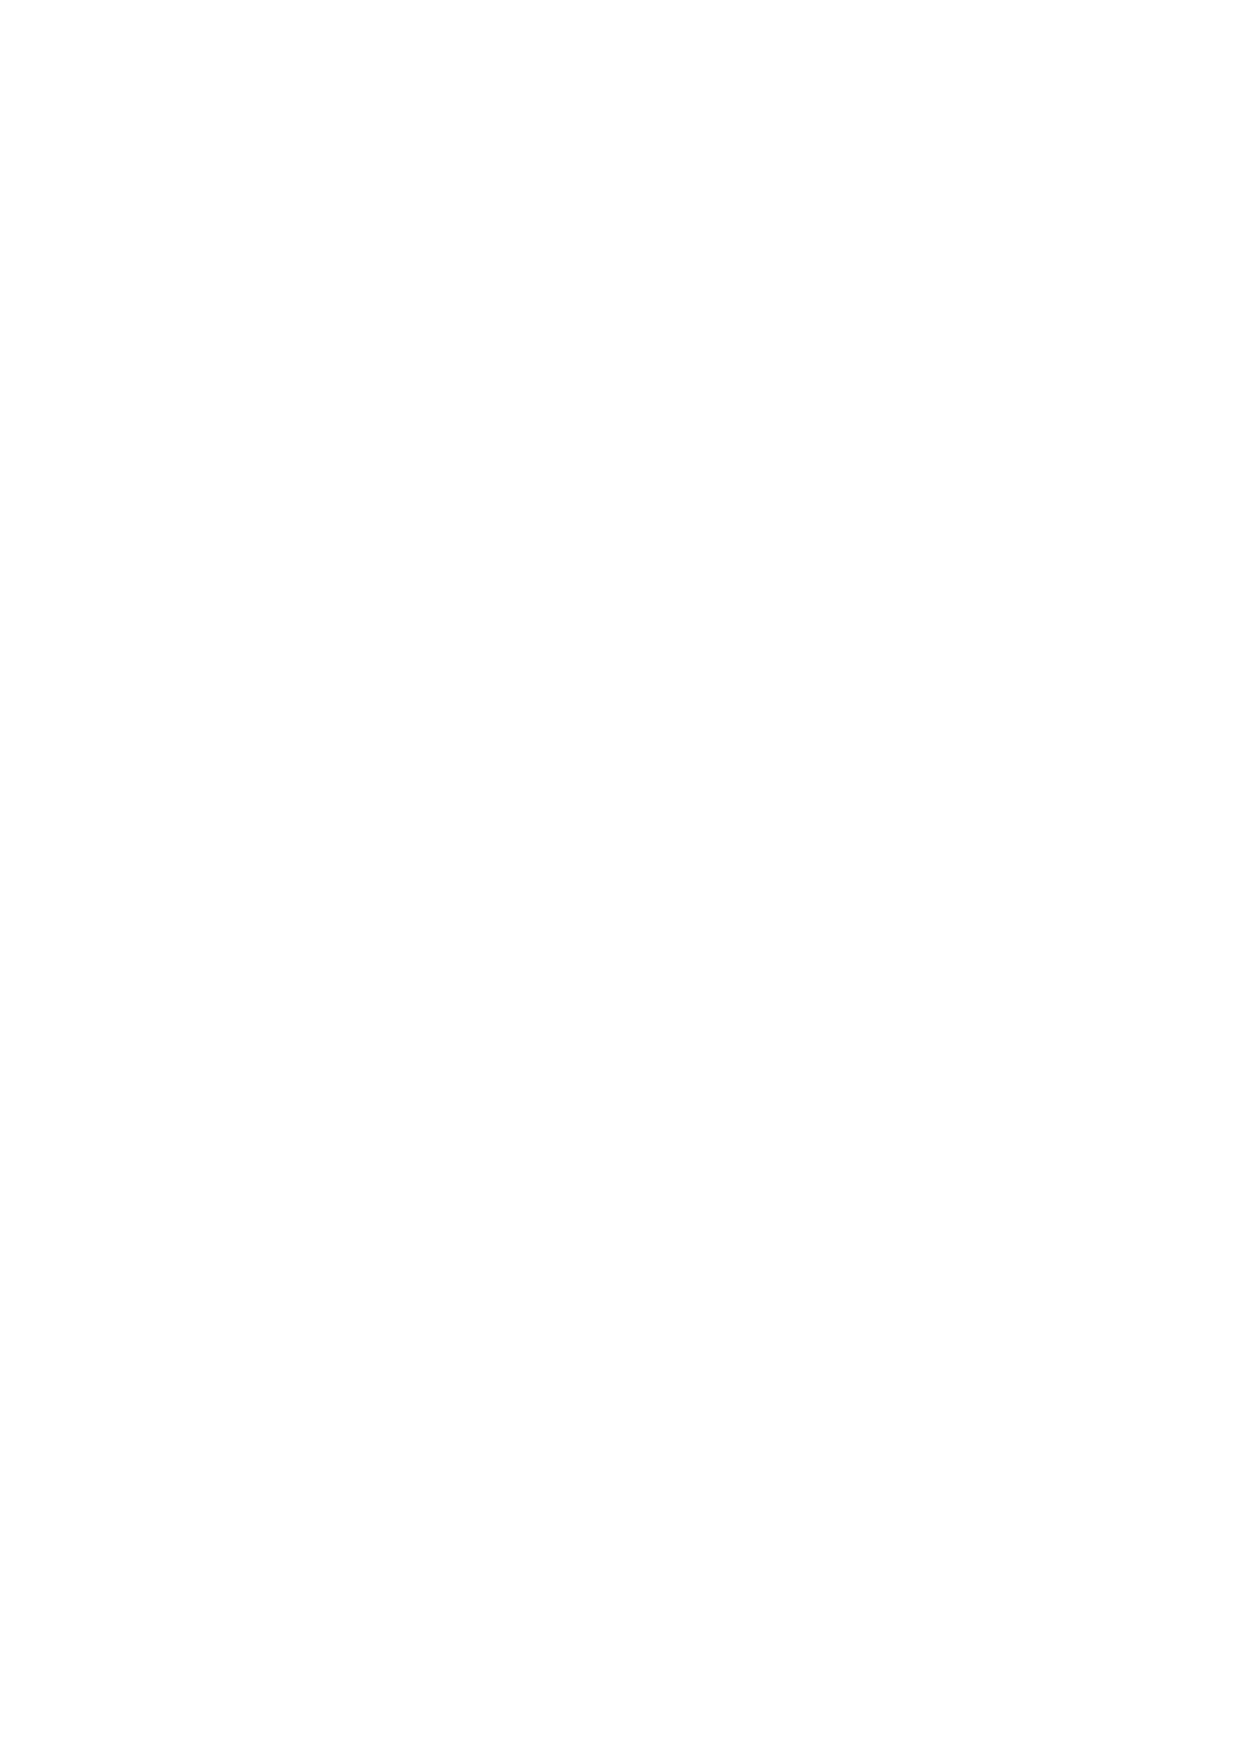
\includegraphics [scale=1.4]{jtr41}
	\caption{The dynamics are quasi-periodic on a torus.}
	\label{fig:4.1}
\end{figure}

\begin{example}
	For the Van der Pol system with $\varepsilon =0$ and $H=%
	\frac{1}{2}(x^{2}+y^{2})$, the action-angle variables are: $I=H$ and $\varphi =\arg (x+iy).$
	
	Consider now the following perturbation of system \eqref{4.3}
	\begin{equation}
	\label{4.4}
	\dot{I}=\varepsilon g(I,\varphi ),\text{ \ \ }\dot{\varphi}=\omega
	(I)+\varepsilon f(I,\varphi ),
	\end{equation}
	where $I=(I_{1},\ldots ,I_{n}),$ $\varphi =(\varphi _{1},\ldots ,\varphi
	_{n})$\ and $\omega =\left( \omega _{1},\ldots ,\omega _{n}\right) $.
	It is natural to expect that the solution of the system \eqref{4.4} after time of order $O(1)$ differs from the solution of the system \eqref{4.3} with the same initial conditions by size of order $O(\varepsilon )$. Meanwhile, Theorem \ref{theo:4.4} says that the same size $O(\varepsilon )$ can be obtained after a time that tends to infinity at $\varepsilon \rightarrow 0.$ This kind of phenomenon takes place thanks to the so-called averaging.
	
	The idea of averaging is connected with the fact that on the surface of torus $\mathbb{T}^{n}=\left\{ I=d\right\} $ the trajectories of a non-perturbed system are dense (as in Figure \ref{fig:4.1}). Therefore, the average deviation of action $I(t)$ can be calculated (approximately) by averaging on the torus.
\end{example}

We define the average system
\begin{equation}
\label{4.5}
\dot{J}=\varepsilon G(J),
\end{equation}
where
$$
G(J)=\left( \frac{1}{2\pi }\right) ^{n}\int_{0}^{2\pi }\ldots \int_{0}^{2\pi
}g(J,\varphi )d\varphi _{1}\ldots d\varphi _{n}
$$
is the average of the speed of change of action on $\mathbb{T}^{n}$.

\begin{theorem}\emph{(About averaging).}
	Let $n=1$ and functions $\omega ,f,g$ be of class $C^1$ and $\omega (I)>0$ be an open subset of $\mathbb{R}^{1}\times \mathbb{T}^{1}$. If $\left( I(t),\varphi (t)\right) $ and $\left( J(t),\psi (t)\right) $ are solutions of the systems \eqref{4.4} and \eqref{4.5} such that $I(0)=J(0)$, then for
	$$
	0<t<1/\varepsilon
	$$
	we have
	$$
	\left\vert I(t)-J(t)\right\vert <C\cdot \varepsilon ,
	$$
	where constant $C$ depends only on $\omega ,f,g.$
	\begin{proof}
		Let's replace
		\begin{equation}
		\label{4.6}
		K=I+\varepsilon k(I,\varphi )
		\end{equation}
		so that there is $\dot{K}=O(\varepsilon ^{2})$. The calculation $k(J,\varphi
		)$ follows form the following
		$$
		\begin{array}{lll}
		\dot{K} &=&\dot{I}+\varepsilon \frac{\partial k}{\partial I}\dot{I}%
		+\varepsilon \frac{\partial k}{\partial \varphi }\dot{\varphi}=\varepsilon
		\left\{ g+\frac{\partial k}{\partial \varphi }\omega \right\} +O(\varepsilon
		^{2}) \\
		&=&\varepsilon \left\{ g(K,\varphi )+\frac{\partial k}{\partial \varphi }%
		(K,\varphi )\omega (K)\right\} +O(\varepsilon ^{2}).
		\end{array}
		$$
		So we want to solve the equation
		$$
		\frac{\partial k}{\partial \varphi }(K,\varphi )\omega (K)=-g(K,\varphi),
		$$
		with the obvious solution $g(K,\varphi )=\frac{-1}{\omega (K)}%
		\int_{0}^{\varphi }g(K,\psi )d\psi .$  Unfortunately, usually this solution is not an explicit (or periodic) function from $\varphi$. The obstacle is the quantity $\int_{0}^{2\pi }g(h,\psi )d\psi$, which can be non-zero.
		
		But, by writing
		$$
		g(K,\varphi )=G(K)+\tilde{g}(K,\varphi )
		$$
		so that $\int_{0}^{2\pi }\tilde{g}(h,\psi )d\psi =0$, we can define the unambiguous functions
		$$
		g(K,\varphi )=\frac{-1}{\omega (K)}\int_{0}^{\varphi }\tilde{g}(K,\psi)d\psi .
		$$
		We get the equation
		$$
		\dot{K}=\varepsilon G(K)+O(\varepsilon ^{2}).
		$$
		
		You can see that after the time $O(1/\varepsilon )$ the difference between $J(t)$ and $K(t)$ is of order $O(\varepsilon )$. On the other hand, the difference between $K (t)$ and $I (t)$ is of order $O(\varepsilon )$, thanks to the change \eqref{4.6}.
	\end{proof}
\end{theorem}

For perturbations of type \eqref{4.4} of completely integral Hamiltonian systems with many degrees of freedom of estimation, they are weaker than in the thesis of Theorem \ref{theo:4.4}. It turns out that after time of order $O(1/\varepsilon ^{a})$, for initial conditions outside the set with Lebesque's measure $O(\varepsilon ^{b})$, the deviation $J(t)$ from $I(t)$ does not exceed $O(\varepsilon ^{c})$, where $a, b, c> 0$ are exponents dependent on $\omega ,f,g.$ For more information, I refer the reader to \cite{Ar2}.

\begin{example}\label{example:4.5}
	(Abel integrals). Let's consider the following perturbation of the two-dimensional Hamiltonian system
	$$
	\dot{x}=H_{x}^{\prime }+\varepsilon P(x,y),\text{ \ \ \ }\dot{y}%
	=-H_{x}^{\prime }+\varepsilon Q(x,y).
	$$
	For $\varepsilon =0$, the phase curves lie in the levels of Hamilton function $H (x, y)$. In some area of the phase space these curves are closed.
	As we have already done several times, the study of limit cycles of the perturbed system consists in analyzing the transformation of Poincaré's return from $S$ (transversal cut to phase curves) to $S$. Parameterizing $S$ with $H|_{S}$ the boundary cycle condition is $\Delta H=H(B)-H(A)=0$ (see Figure \ref{fig:4.2}). We have
	$$
	\begin{array}{lll}
	\Delta H &=&\int_{0}^{T}\frac{dH}{dt}dt=\int_{0}^{T}\left\{ H_{x}^{\prime
	}\left( H_{y}^{\prime }+\varepsilon P\right) +H_{y}^{\prime }(-H_{x}^{\prime
	}+\varepsilon Q\right\} dt \\
	&=&\varepsilon \int \left( PH^{\prime }x+QH_{y}^{\prime }\right)
	dt=\varepsilon \int \left\{ P(H_{x}^{\prime }-\varepsilon Q)+Q\left(
	H_{y}^{\prime }+\varepsilon P\right) \right\} \\
	&=&\varepsilon \int_{\Gamma (h)}Qdx-Pdy=\varepsilon \oint_{H=h}\left(
	Qdx-Pdy\right) +O(\varepsilon ^{2}),
	\end{array}
	$$
	where $T$ is the time to return to $S$ and $\Gamma (h)$ is the phase curve of the perturbed system starting from $A\in S$ such that $H (A) = h$.
	\begin{figure}[!ht]
		\centering
		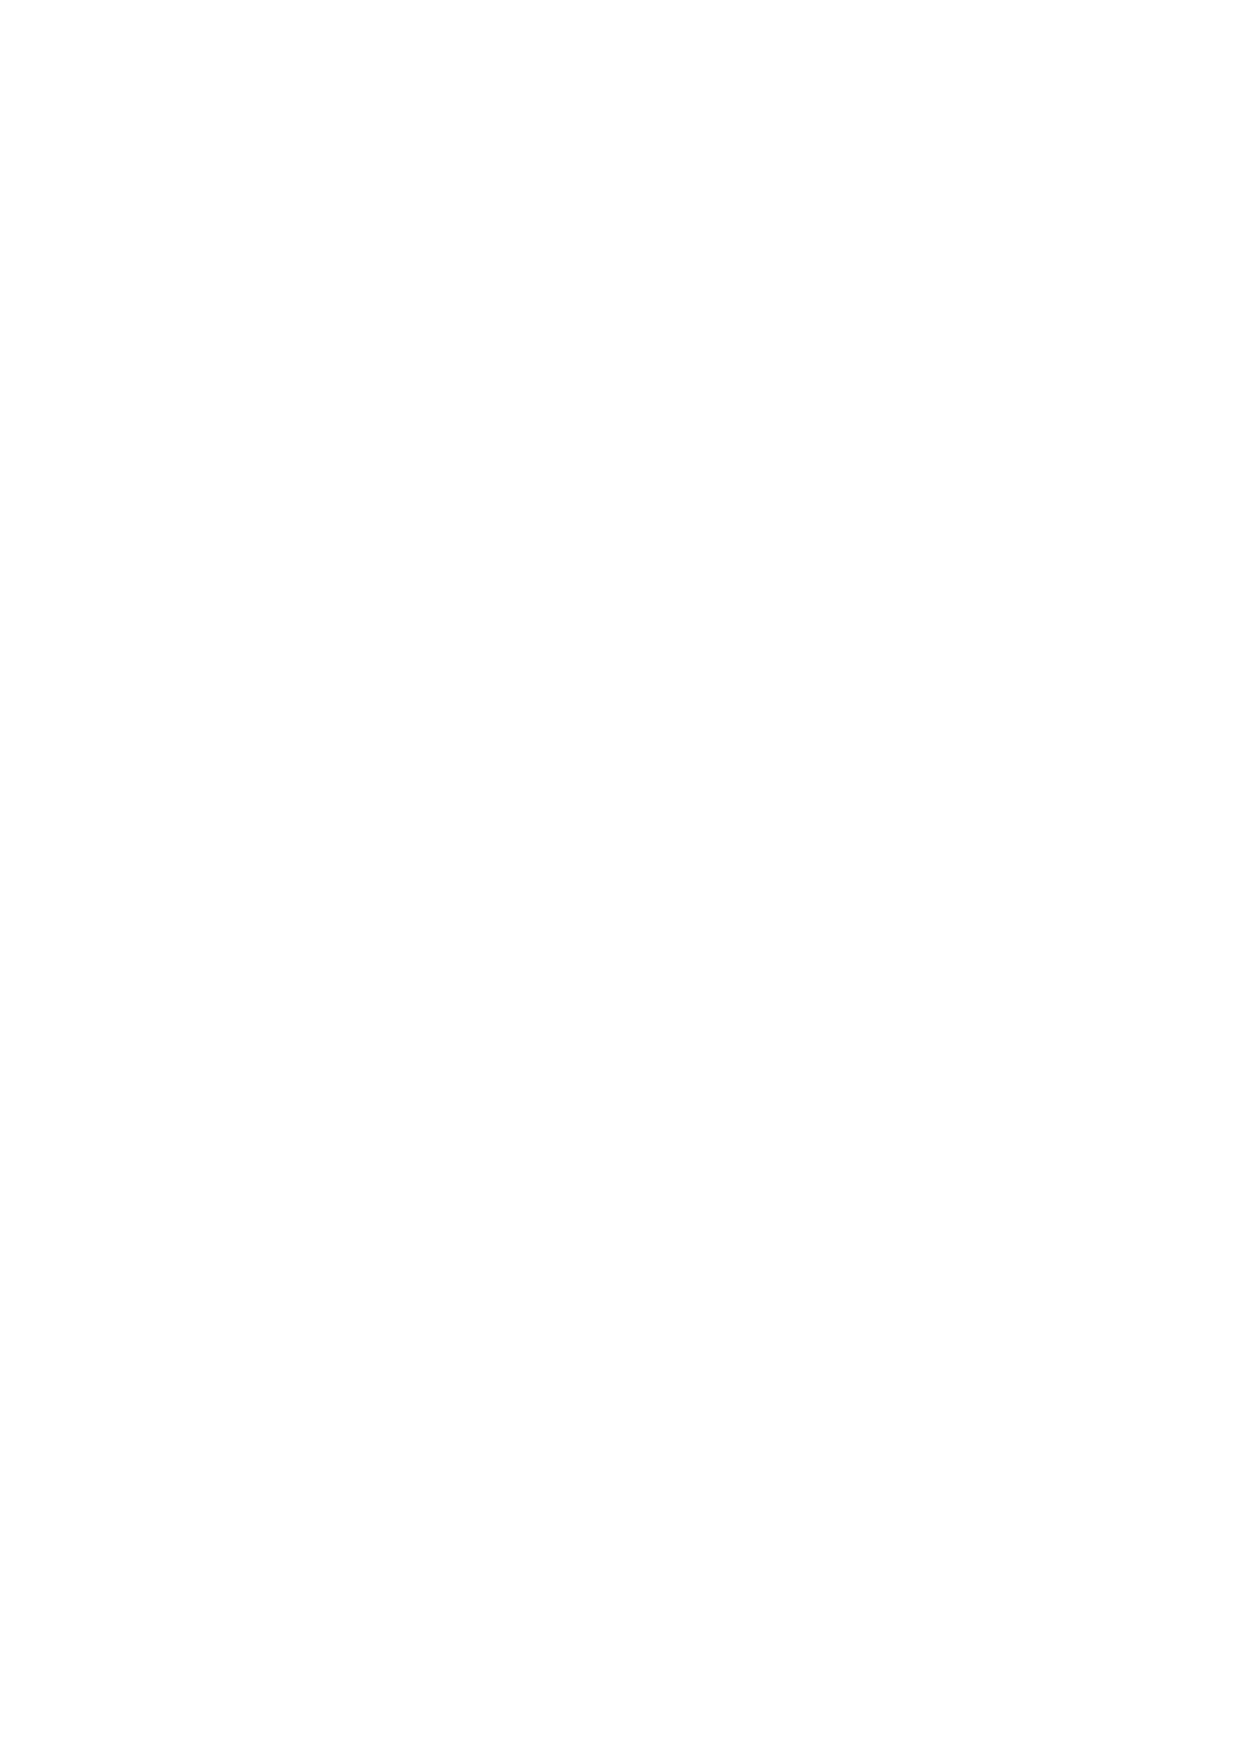
\includegraphics [scale=1.4]{jtr42}
		\caption{Conversion of a return map to the perturbed Hamiltonian system.}
		\label{fig:4.2}
	\end{figure}

	The expression
	\begin{equation}
	\label{4.7}
	I(h)=\oint_{H=h}Qdx-Pdy
	\end{equation}
	is so-called \textbf{Abel's integral}.\footnote{The concept of the abelian integral derives from the complex algebraic geometry. They are integrals of meromorphic 1-forms along certain closed curves on complex algebraic curves (Riemann surfaces). When $H(x,y),$ $P(x,y)$ and $Q(x,y)$ are polynomials, then the Riemann surface is the complex curve $\left\{ H(x,y)=h\right\} \subset \mathbb{C}^{2}$ and the 1-form is $\omega = \left( Qdx-Pdy\right) |_{H=h}.$} Theorems about implicit functions result from the fact that if $I(h_{0})=0$ and $I^{\prime }(h_{0})\not=0$, then for small $\varepsilon \not=0$ and small there is a limit cycle $\gamma_{\varepsilon }$, which strokes the curve $H=h_{0}$ as $\varepsilon \rightarrow 0$. This approach to the problem of limit cycles is widely used in the Qualitative Theory.

	It is not difficult to notice that the function $I(h)$ is the equivalent of the integral of $G(J)$, which occurs in the formula \eqref{4.5}.
\end{example}

\section{KAM Theory}
Consider the Hamiltonian system
$$
\dot{q}=H_{p}^{\prime },\text{ \ \ \ }\dot{p}=-H_{q}^{\prime },
$$
$p=\left( p_{1},\ldots ,p_{n}\right) ,$ $q=\left( q_{1},\ldots ,q_{n}\right)$, with the Hamiltonian form
$$
H(p,q)=H_{0}(p,q)+\varepsilon H_{1}(p,q),
$$
where $H_{0}$ is the Hamiltonian of a completely integer system, i.e. a system of type \eqref{4.3} in action-angle variables. This situation is connected with one of the most important mathematical theorems of the second half of the XX century. Before formulating it, we have to introduce two more assumptions regarding the non-degeneration of the unperturbed $H_0$ Hamiltonian:
\begin{equation}
\label{4.8}
\det \left( \frac{\partial \omega _{i}}{\partial I_{j}}\right) =\det \left(
\frac{\partial ^{2}H_{0}}{\partial I_{i}\partial I_{j}}\right) \not=0,
\end{equation}%
\begin{equation}
\label{4.9}
\det 
\begin{pmatrix}
\frac{\partial ^{2}H_{0}}{\partial I_{i}\partial I_{j}} & \frac{\partial
	H_{0}}{\partial I_{i}} \\
\frac{\partial H_{0}}{\partial I_{j}} & 0%
\end{pmatrix} \neq 0.
\end{equation}

The condition \eqref{4.8} means that frequencies $\omega _{i}(I)$ will become independent and fit quickly with the change of actions $I_{j}$, while the condition \eqref{4.9} means that these frequencies change quickly and independently, after limitation to the levels $\left\{ H_{0}=\textrm{const}\right\}$.

\begin{theorem}\emph{(Kolmogorov–Arnold–Moser).}
	If the non-degeneration conditions \eqref{4.8} and \eqref{4.9} are satisfied for $H_{0}$, then for a small perturbation $H=H_{0}+\varepsilon H_{1}$ most of the invariant torus ${I = \textrm{const}}$ do not disappear, but only slightly deforms and movement on them are still quasi-periodic.
\end{theorem}

This theorem was formulated in 1954 at the International Congress of Mathematicians in Amsterdam, but it had to wait for the strict proof until the beginning of the sixties. It was given by V. Arnold (in the analytical case) and J. Moser (in the case of a smooth of class $C^{333}$). The smoothness class was later reduced to $C^3$. Of course I am not able to present this proof here.

\begin{example} (The flat limited problem of three bodies).
	The \textbf{flat limited problem of the three bodies} is a system in which two bodies (interacting forces of gravity) rotate at a constant angular velocity around their center of mass (at the beginning of the coordinate system) and the third body moves in the plane of rotation of two bodies and has a mass so small that it does not interfere with their movement. In Figure \ref{fig:4.3} we have a system in which $S$ means Sun, $J$ means Jupiter, and $A$ is an Asteroid. Units of time, length and mass can be chosen so that the angular velocity, the sum of  the masses of $S$ and $J$ and the gravitational constant are equal to 1. Then the distance between $S$ and $J$ also equals 1. The only parameter characterizing the system is the mass of Jupiter $\mu$.
	
	The Asteroid motion equations are Hamiltonian with the Hamiltonian
	$$
	\frac{1}{2}(p_{1}^{2}+p_{2}^{2})-\frac{1-\mu }{\rho _{1}}-\frac{\mu }{\rho_{2}},
	$$
	where $\rho _{1}$ and $\rho _{2}$ are the distances $A$ from $S$ and $J$, respectively. Note that the positions $S$ and $J$ change over time: $J=\left( 1-\mu \right) (\cos t,\sin t),$\ $S=(-\mu
	)\left( \cos t,\sin t\right)$; therefore, the Hamiltonian depends directly on time.
	\begin{figure}[!ht]
		\centering
		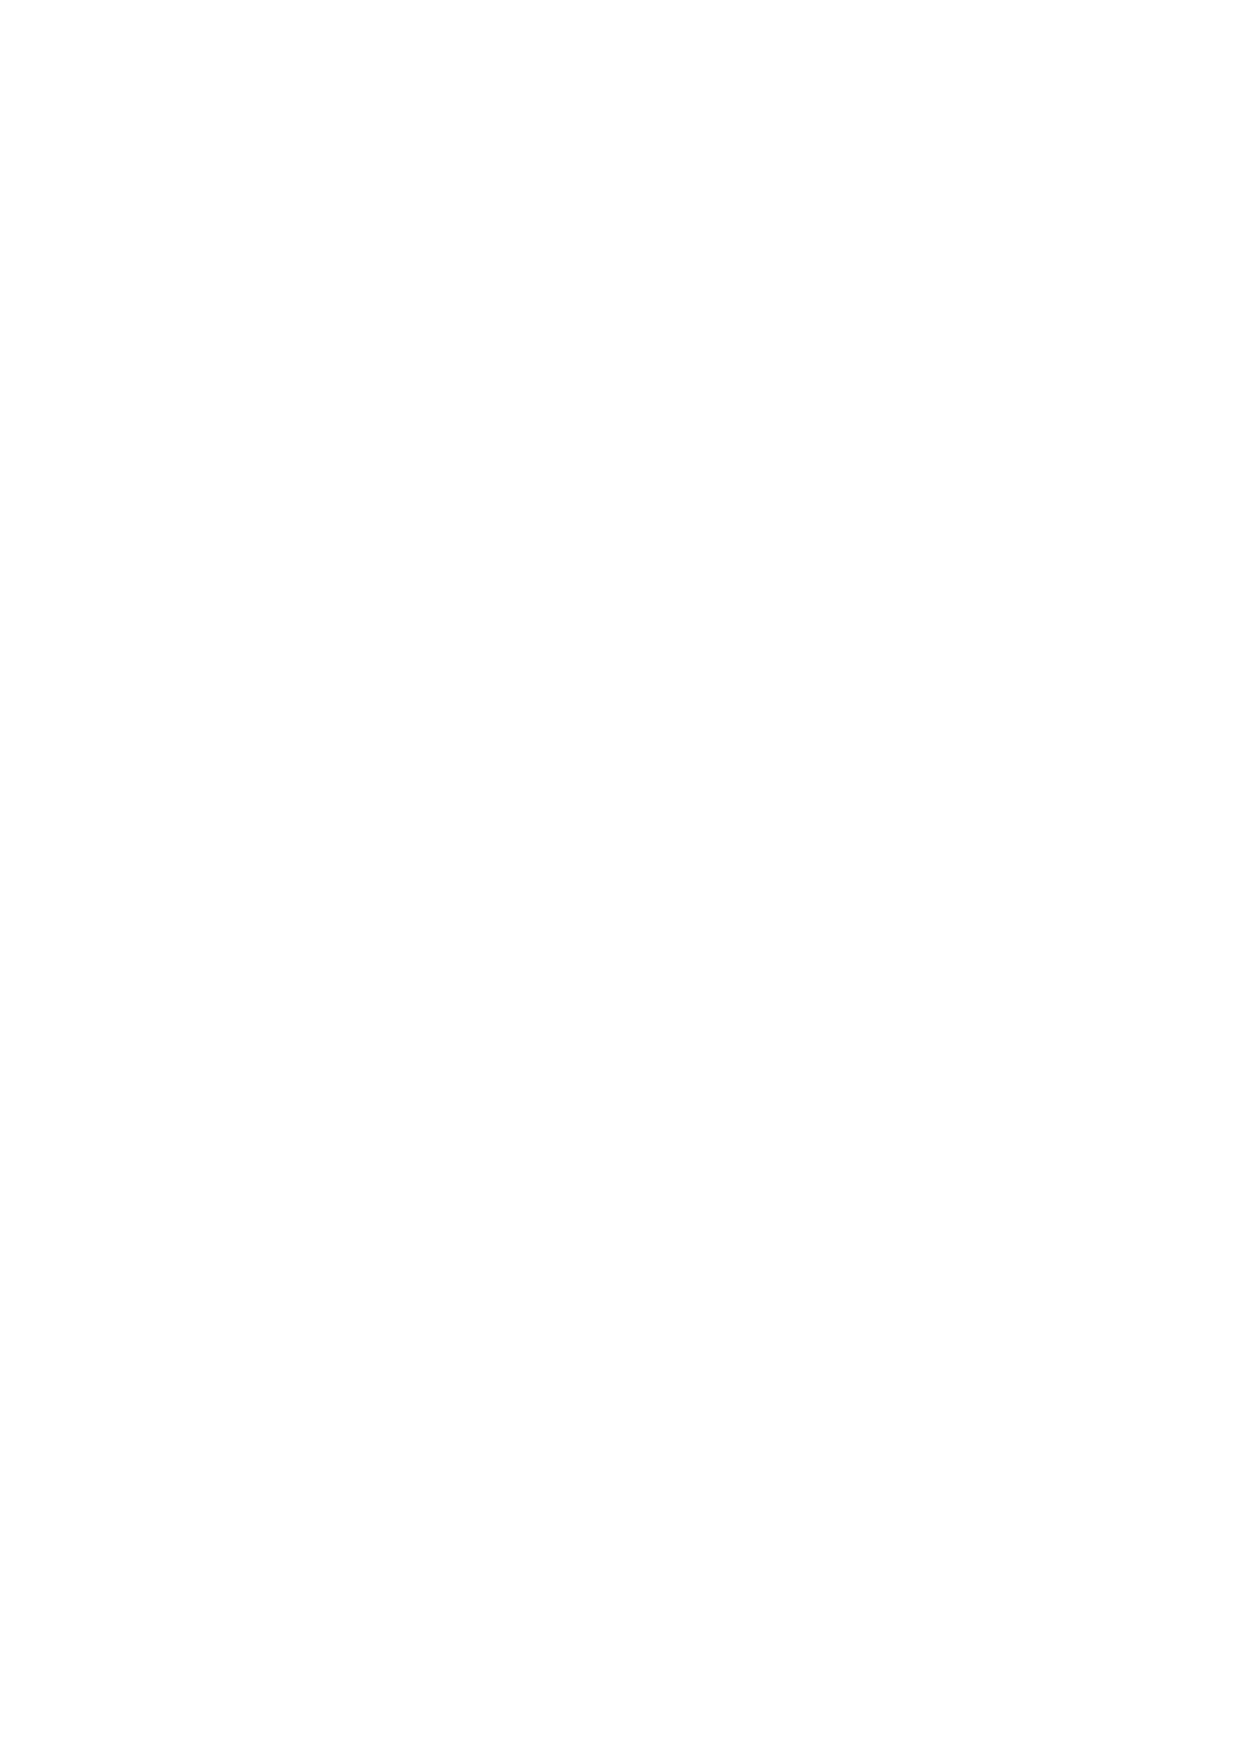
\includegraphics [scale=1.4]{jtr43}
		\caption{The problem of three bodies and invariant torus.}
		\label{fig:4.3}
	\end{figure}

	To get rid of this dependence on time, we make the following change (simultaneous rotation of coordinates and sprouts)
	$$
	q^{\prime }=M(t)q,\text{ \ \ }p^{\prime }=M(t)p,\text{ \ \ }M(t)=\left(
	\begin{array}{ll}
	\cos t & \sin t \\
	-\sin t & \cos t%
	\end{array}%
	\right) .
	$$
	It turns out that the new variables are still Hamiltonian with the new Hamiltonian
	\begin{equation}
	\label{4.10}
	H =\frac{1}{2}\left( p_{1}^{\prime }+q_{2}^{\prime }\right) ^{2}+\frac{1}{2%
	}\left( p_{2}^{\prime }-q_{1}^{\prime }\right) ^{2}-V(q_{1}^{\prime
	},q_{2}^{\prime }),
	\end{equation}
	
	$$
	V =\frac{q_{1}^{\prime 2}+q_{2}^{\prime 2}}{2}+\frac{1-\mu }{\rho _{1}}+%
	\frac{\mu }{\rho _{2}},
	$$
	$\rho _{1}^{2}=\left( q_{1}^{\prime }+\mu \right) ^{2}+q_{2}^{\prime 2}$, $\rho _{2}^{2}=\left( q_{1}^{\prime }+\mu -1\right) ^{2}+q_{2}^{\prime 2}$ (Task 4.13). In the new variables $q_{1}^{\prime }$, $q_{2}^{\prime }$, the bodies $S$ and $J$ are resting.
	
	The Hamiltonian's system equilibrium points are the critical points of the Hamiltonian function (Task 4.14). In the case of Hamiltonian \eqref{4.10}, these points, which we call \emph{relative positions of equilibrium}, are given by 
	$$
	p_{1}^{\prime }=-q_{2}^{\prime },\text{ \ \ }p_{2}^{\prime }=q_{1}^{\prime },%
	\text{ \ \ }\partial V/\partial q_{1}^{\prime }=\partial V/\partial
	q_{2}^{\prime }=0.
	$$
	We have
	\begin{eqnarray*}
		\frac{\partial V}{\partial q_{2}^{\prime }} &=&q_{2}^{\prime }\left( 1-\frac{%
			1-\mu }{\rho _{1}^{3}}-\frac{\mu }{\rho _{2}^{3}}\right) =q_{2}^{\prime }f,
		\\
		\frac{\partial V}{\partial q_{2}^{\prime }} &=&q_{1}^{\prime }f-\mu (1-\mu
		)\left( \frac{1}{\rho _{1}^{3}}-\frac{1}{\rho _{2}^{3}}\right) .
	\end{eqnarray*}
	We have two options:
	\begin{enumerate}
		\item $q_{2}^{\prime }=0$; here we find three points of the so-called \emph{collinear liberty points} $L_{1}$, $L_{2}$, $L_{3}$	(Task 4.15), which are unstable.
		\item $f=0$ and $\rho _{1}=\rho _{2}=1$; here we have two so-called \emph{triangular points of liberty} $L_4$ and $L_5$, which lies in the vertices of two equilateral triangles with a base $\overline{SJ}.$
	\end{enumerate}

	Calculations that we do not carry out show that for $27\mu
	(1-\mu )>1$, $L_{4,5}$ points are unstable whereas in the opposite case, i.e. for $\mu <\mu _{1}=\frac{1}{2}(1-\sqrt{23/27})\approx 0.03852$, the eigenvalues of the linear part of the Hamiltonian system are in the form $\pm i\omega _{1}$, $\pm i\omega _{2}$, where $\omega _{1}<0<\omega _{2}\not=\omega _{1}$. We are on the border of the stability area.
	
	In addition, the square part of $H$ at point $L_{4}$ takes the form
	$$
	H_{0}=\frac{1}{2}\omega _{1}(\tilde{p}_{1}^{2}+\tilde{q}_{1}^{2})+\frac{1}{2}%
	\omega _{2}\left( \tilde{p}_{2}^{2}+\tilde{q}_{2}^{2}\right)
	$$
	in the appropriate coordinate system in the neighborhood of $L_{4}$ (see \cite{Zol1}). It is a completely integrable Hamiltonian system with a change in action-angle $I_{1}=\frac{1}{2}(\tilde{p}_{1}^{2}+\tilde{q}%
	_{1}^{2})$, $I_{2}=\frac{1}{2}\left( \tilde{p}_{2}^{2}+\tilde{q}%
	_{2}^{2}\right) $, $\varphi _{1}=\arg \left( \tilde{q}_{1}+i\tilde{p}%
	_{1}\right) $, $\varphi _{2}=\arg \left( \tilde{q}_{2}+i\tilde{p}%
	_{2}\right) $ and with $H_{0}=\omega _{1}I_{1}+\omega _{2}I_{2}$ (Task 4.16).
	
	We have situations like in KAM theorem: $H=H_{0}+H_{1}$, where $H_0$ is completely integrable and $H_1$ contains terms of order $> 2$ due to $I_{j}$ (which are small). Unfortunately, this is not enough because the frequencies of $\omega _{j}=\partial H_{0}/\partial I_{j}$ are constant, and from the condition of non-degeneration \eqref{4.8} should change with $I_{j}$. Therefore, we should take into account further terms of the $H$ expansion in the $L_4$ neighborhood.
	
	More specifically, we simplify the terms of the third and fourth order in the Hamiltonian $H$. This simplification is an analogue of Poincaré-Dulac's normal form and has been proved by G. Birkhoff in Theorem \ref{theo:4.9} below. This \emph{Birkhoff normal form} in our case has the following form
	\begin{equation}
	\label{4.11}
	H=H_{0}+H_{1},\text{ \ }H_{0}=\omega _{1}I_{1}+\omega _{2}I_{2}+\sum \omega
	_{ij}I_{i}I_{j},\text{ \ }I_{j}=\frac{1}{2}(P_{j}^{2}+Q_{j}^{2}),
	\end{equation}
	where $P_{j}=\tilde{p}_{j}+\ldots$, $Q_{j}=\tilde{q}_{j}+\ldots $ are new variables and $H_1$ contains terms of order 5 (and $H_0$ and $H_1$ are different than above). In the assumption of Birkhoff's theorem, there is a condition of no resonant relations of order 4 and 3. It turns out that such relations occur for the values of $\mu_{2}=\frac{1}{2}\left( 1-\sqrt{1833}/45\right) \approx 0.02429$ and $\mu _{3}=\frac{1}{2}\left( 1-\sqrt{213}/15\right) \approx 0.01352$; therefore, these values of the $\mu$ parameter should be excluded.
	
	Hamiltonian $H_{0}=H_{0}(I_{1},I_{2})$ is a completely integrable Hamiltonian and has a chance of satisfying non-degeneration conditions \eqref{4.8} and \eqref{4.9}. It turns out that only condition \eqref{4.9} is significant. A. Leontovych showed that it can be violated only for a discrete set of values of parameter $\mu$.\footnote{In \cite{Zol1} one can find out that the condition \eqref{4.9} is violated for adding one specific value of the $\mu$ parameter. This value resulted from the formula for the determinant in equation \eqref{4.9} given by the French astronomers A. Deprit and A. Deprit-Bartholomé (and cited in very serious monographs). Recently, with my graduate student W. Barwicz, we discovered that this pattern is not true, and even contrary to the calculations of Leontovych. In fact, the determinant is a very complicated algebraic function from $\mu$, which is not identical to zero.} Let us assume then that $\mu$ satisfies all the conditions listed above, which is the real thesis of KAM theorem.
	
	How does stability result from the KAM theorem? Well, we are in a 4-dimensional space surrounded by an equilibrium point. Because the system is Hamiltonian with the Hamiltonian independent of time, so the movement takes place on the surfaces $H=\textrm{const}$. They are three-dimensional. From the KAM theorem, it follows that every such surface is almost filled with the invariant torus $\mathbb{T}^{2}$, which is the more we are closer to the torus $I_{1}=I_{2}=0$. Each invariant torus breaks down the $H=\textrm{const}$ surface into two parts, its interior and exterior. No interior point comes out of it during evolution. Because in the space of P, Q variables, toruses can be arbitrarily small, this results in stability in the sense of Lyapunov.
\end{example}

We will complete the above example. Let's assume we have a Hamiltonian in the form
$$
H=\sum \omega _{j}\cdot \frac{1}{2}(p_{j}^{2}+q_{j}^{2}) + \ldots .
$$

\begin{definition}
	We say that the `frequencies' $\omega _{j}$ satisfies the \textbf{resonance relations of order} $d$, if there are integers $k_{1},\ldots ,k_{n}$ with $\sum \left\vert
	k_{j}\right\vert =d$ such that
	$$
	\sum k_{j}\omega _{j}=0.
	$$
\end{definition}

\begin{theorem}\label{theo:4.9}\emph{(Birkhoff).}
	If the frequencies $\omega _{j}$ do not satisfy any resonant relation of order $\leq 2m$, then there is a canonical exchange of variables $\left( p,q\right) \longmapsto \left( P,Q\right) =\left( p+\ldots ,q+\ldots
	\right) $ leading to the Hamiltonian
	$$
	H=\sum_{\left\vert l\right\vert \leq m}a_{l}I^{l}+O\left( \left\vert \left(
	p,q\right) \right\vert ^{2m+1}\right) ,
	$$
	where $I_{j}=\frac{1}{2}(P_{j}^{2}+Q_{j}^{2})$ and the summation runs along the $\left( l_{1},\ldots
	,l_{n}\right) $ multi-planes with $\left\vert l\right\vert =l_{1}+\ldots +l_{n}$ and $I^{l}=I_{1}^{l_{1}}\ldots I_{n}^{l_{n}}$.
\end{theorem}

\begin{remark}
	Conversion $\left( p,q\right) \longmapsto \left(P,Q\right) $, occurring in the above theorem is canonical if
	$$
	\sum dp_{j}\wedge dq_{j}=\sum dP_{j}\wedge dQ_{j}.
	$$
	It turns out that after the canonical exchange of variables, the Hamiltonian system changes into the Hamiltonian system (see \cite{Ar3}).
\end{remark}

\subsection*{Tasks}
\begin{task}
	Show that if the Hamilton function $H$ does not depend directly on time, it is the first integral for the system \eqref{4.2}.
\end{task}

\begin{task}
	Show that the vector field given by the formula \eqref{4.2} has zero divergence. Deduce the form that the corresponding phase stream keeps its volume.
\end{task}

\begin{task}
	Prove formula \eqref{4.10}.
\end{task}

\begin{task}
	Show that if $H$ does not depend directly on time, the equilibrium points of the system \eqref{4.2} are exactly critical points of the function $H$.
\end{task}

\begin{task}
	Show that there are exactly three collinear libration points.
\end{task}

\begin{task}
	Show that the Hamiltonian form $H_{0}=\omega
	_{1}I_{1}+\omega _{2}I_{2}$ (or as in formula \eqref{4.11}) is the Hamiltonian of a completely integrable system.
\end{task}

\begin{task}
	Apply the abelian integrals method (Example \ref{example:4.5}) to show that the van der Pol system $\dot{x}=y$, $\dot{y} = -x-a(x^{2}-1)y$ for the small parameter $a> 0$ has exactly one boundary cycle.
\end{task}

\section{Relaxation oscillations (slow-fast systems)}
Let's start with a known example.
\begin{example}(Van der Pol system).
	$$
	\dot{x}=y-x^{3}+x,\text{ \ \ }\dot{y}=-\varepsilon x.
	$$
	(When $\varepsilon =1$ and place $y_{1}=y-x^{3}+x$, then it gets $\dot{x}=y_{1}$, $\dot{y}_{1}=-x-(3x^{2}-1)y_{1}$; exact to scale it is the system from Example \ref{example:2.35}
	\begin{figure}[!ht]
		\centering
		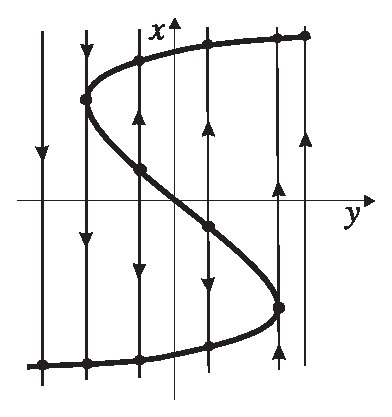
\includegraphics [scale=1.4]{jtr44}
		\caption{The Van der Pol system	`slow-fast' type.}
		\label{fig:4.4}
	\end{figure}
	
	You can see that $x$ changes quickly compared to $y$; we say that $x$ is a \emph{fast variable} and $y$ is \emph{slow}. For $\varepsilon =0$ we have $y = \textrm{const}$ and in fact we have the equation for $x$ dependent on the parameter $y$	(theory of bifurcation bows, see Figure \ref{fig:4.4}). When $\varepsilon \not=0$ (but small), physicists would say that the parameter $y$ `flows'. It is expected that there will be a limit cycle $\gamma _{\varepsilon }$ (in fact $\gamma _{\varepsilon }$ is stable) to the slices of the smooth curve $\gamma_0$ shown in Figure \ref{fig:4.5}. The $\gamma _0$ cycle consists of:
	\begin{itemize}
		\item pieces of slow motion along the curve $y=x^{3}-x$ (where $\dot{x}=0$),
		\item sections of a jump along the straight $y = \textrm{const}$.
	\end{itemize}

	Such movement is an example of relaxation oscillations (like a heartbeat).
	\begin{figure}[!ht]
		\centering
		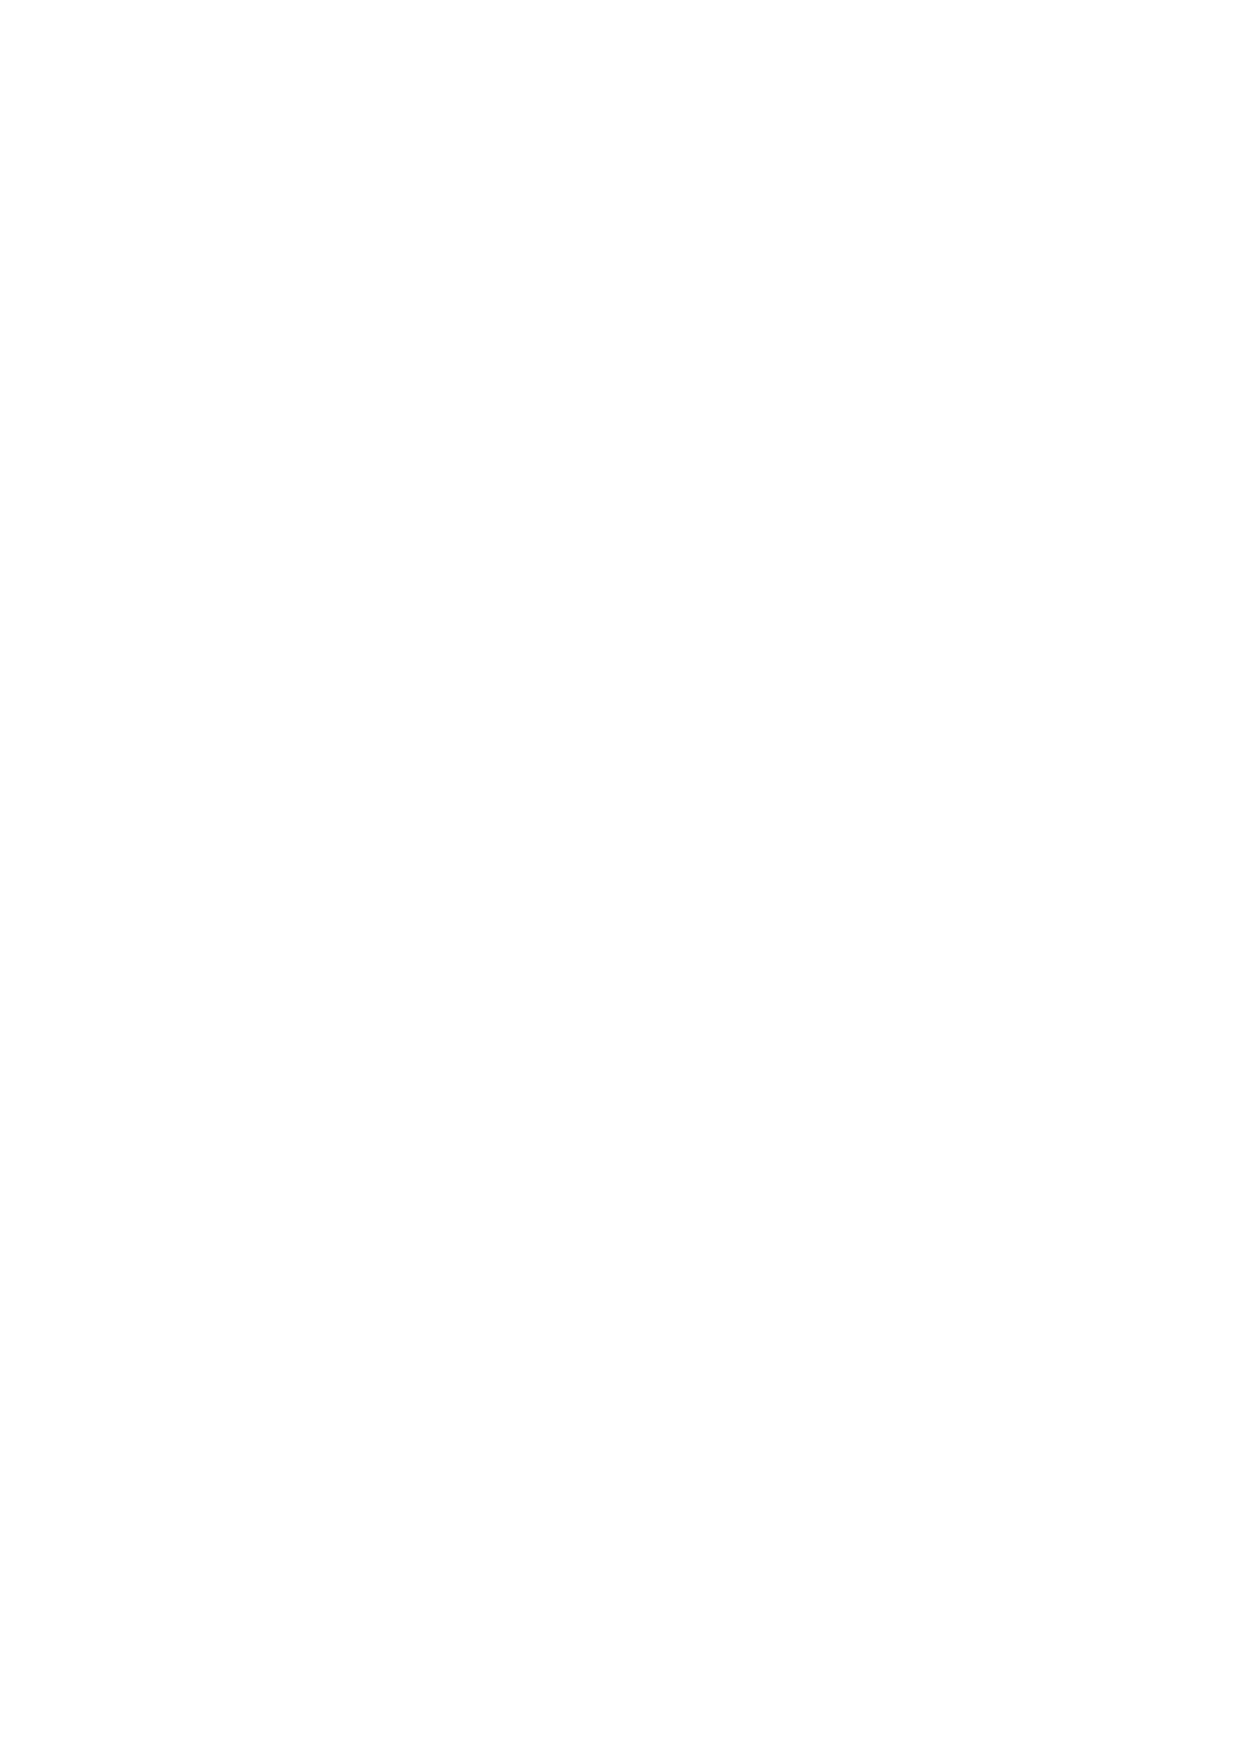
\includegraphics [scale=1.4]{jtr45}
		\caption{Relaxation oscillations.}
		\label{fig:4.5}
	\end{figure}
\end{example}

Consider now the general situation. We have an \textbf{unperturbed system}
$$
\dot{x}=f(x,y),\text{ \ \ \ }\dot{y}=0,
$$%
($x\in \mathbb{R}^{k}$, $y\in \mathbb{R}^{l}$); here $x$ are the \textbf{fast coordinates} and $y$ are the \textbf{slow coordinates}. We also have the \textbf{perturbed system}
$$
\dot{x}=F(x,y;\varepsilon ),\text{ \ \ }\dot{y}=\varepsilon
G(x,y;\varepsilon ),\text{ \ \ \ }F(x,y;0)=f(x,y).
$$

\begin{definition}
	The surface $S = {f (x, y) = 0}$ is called  \textbf{slow surface}.
	
	The slow surface is divided into \textbf{areas of stability} and \textbf{instability} of the undisturbed system; they correspond to situations when $\textrm{Re}\lambda _{j}(A)<0$, $j=1,\ldots ,k$, $A=\frac{\partial f}{\partial x}$, and when there is $\textrm{Re}\lambda _{j}(A)>0$.
	
	On a slow surface, we have a vector field defined as follows. We take the field
	$$
	\frac{\partial }{\partial \varepsilon }\left( F\partial _{x}+\varepsilon
	G\partial _{y}\right) |_{\varepsilon =0}=f_{1}(x,y)\partial
	_{x}+g(x,y)\partial _{y}
	$$
	at point $\left( x,y\right) \in S$ and project it on $T_{(x,y)}S$ along the variable $y$. This is a \textbf{slow motion field}.
\end{definition}

Let us reminding that at the beginning of this chapter we were saying that relaxation oscillations are characterized by the fact that a small parameter appears on the left side. To find out, we introduce slow time $\tau =\varepsilon t$. Then we get the system
$$
\varepsilon \frac{dx}{d\tau }=f(x,y)+O(\varepsilon ),\text{ \ \ }\frac{dy}{%
	d\tau }=g(x,y)+O(\varepsilon ).
$$
Now the \emph{slow motion equation} to $S$ (locally parameterized by $y$) has the form
$$
\frac{dy}{d\tau }=h(y)+O(\varepsilon )
$$
(with the corresponding function $ h$).

Let's analyze the movement of a typical point $(x_0, y_0)$. It consists of pieces of three types: approaching to the slow surface, movement along the slow surface and movement in the transition area.

\begin{figure}[!ht]
	\centering
	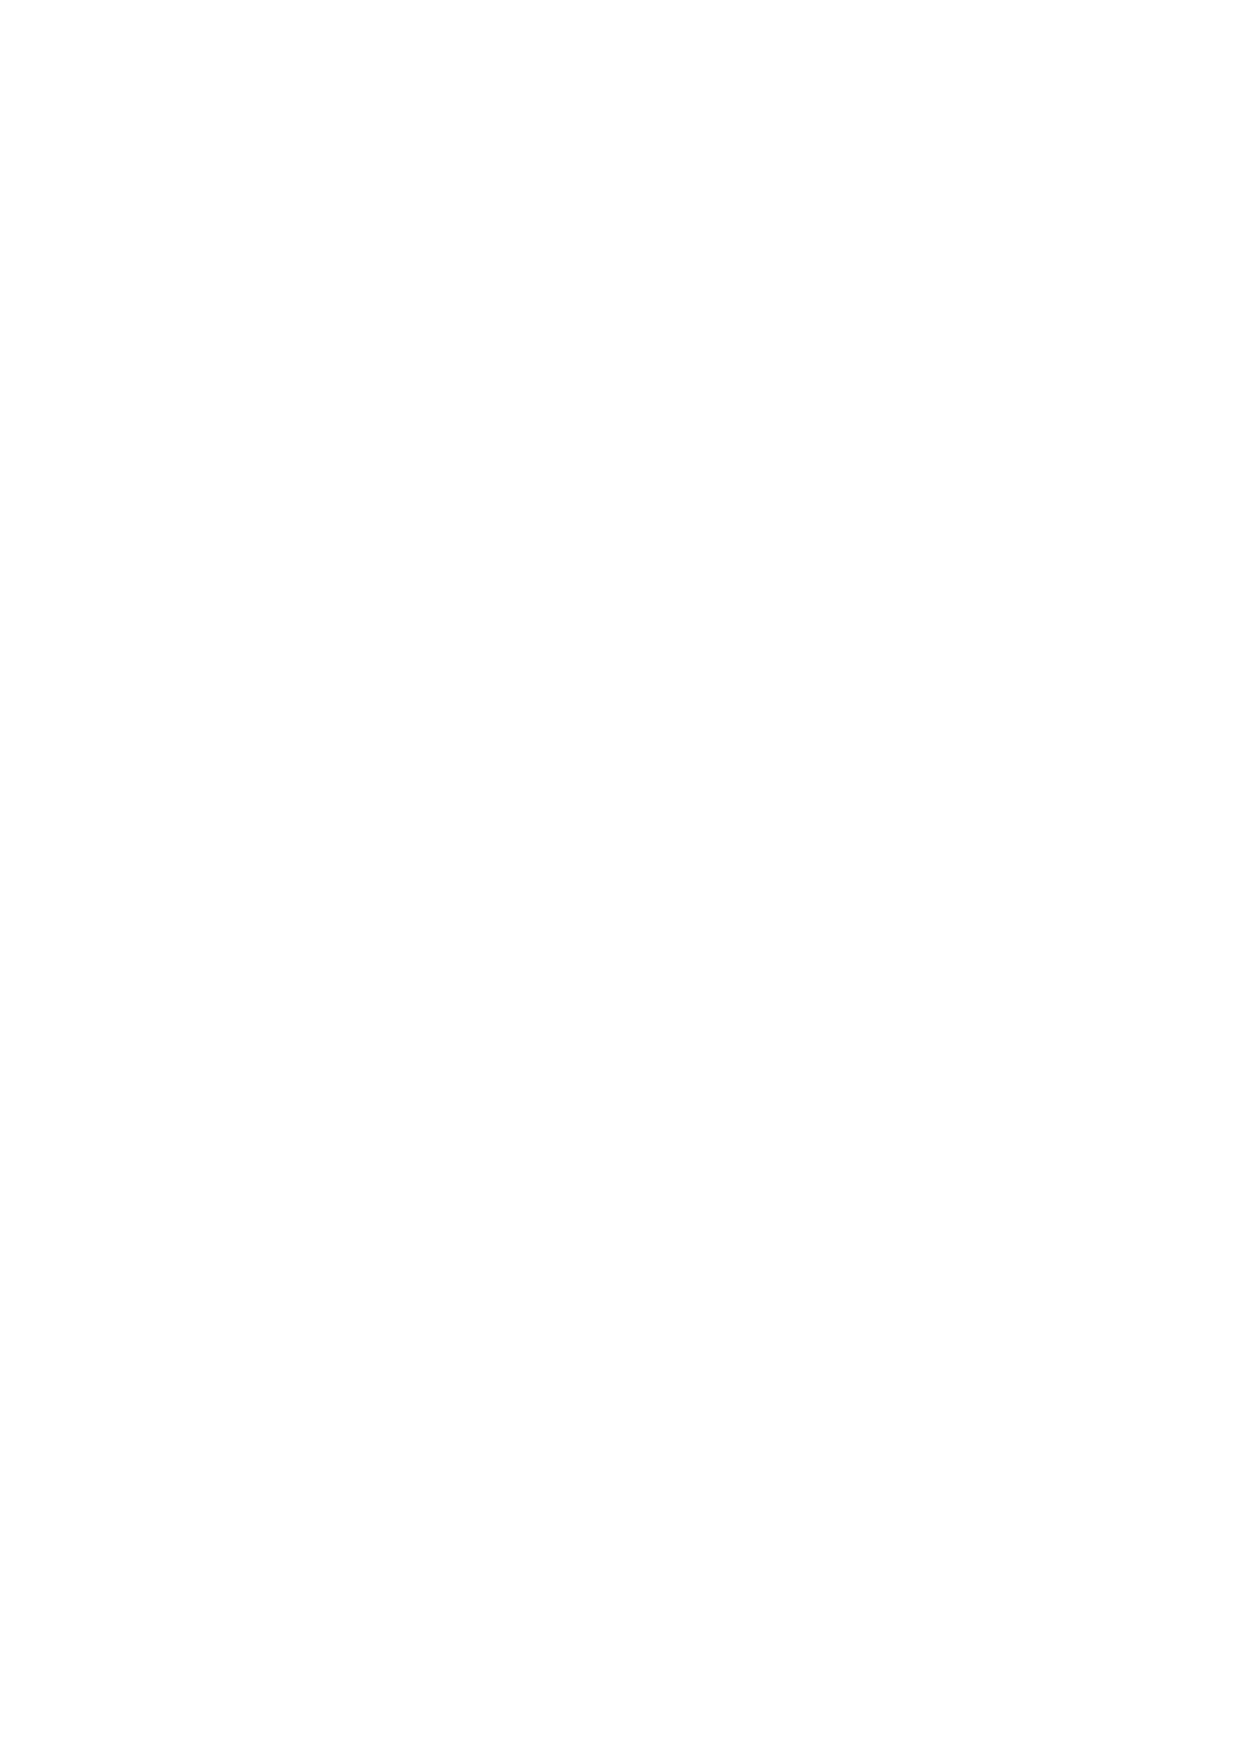
\includegraphics [scale=1.4]{jtr46}
	\caption{Approaching to the slow surface.}
	\label{fig:4.6}
\end{figure}

\subsection{Approaching to the slow surface}
Let the point $(x_0, y_0)$ from outside $S$ be projected (along the $y$ coordinates) to the point $(x_*, y_0)$, $x_* = x_* (y_0)$, to $S$ in the stability area (see Figure \ref{fig:4.6}). This means that point $x_0$ lies in the pool of attraction of the point $x_*$ for the equation $\dot{x} = f (x, y_0)$ ($y_0$ fixed). Consider the area $U = {\left| x - x_* (y_0) \right| <\delta, y_0 \in V}$, where $V$ is a certain area corresponding to a subset of the stability area in $S$. It turns out that the slow recovery time of the solution with the initial condition $(x_0, y_0)$ to $U$ is of order $\tau_1 \sim C_1 \varepsilon \left|\ln \varepsilon\right|$, which corresponds to the actual time
$$
t_1 \sim C_1  \left|\ln \varepsilon\right|
$$
$$
r(t)<C_{1}e^{-C_{2}/\varepsilon }\rightarrow 0,
$$
(constant $C_1$ depends on $U$ and $F$, $G$).

\subsection{Movement along the slow surface}
In the area of $U$, we have slow motion, described by the equation $dy/d\tau =h(y)+O(\varepsilon )$. It lasts until $\tau_{2}=T=O(1)$, which corresponds to the long real time $t_{2}=T/\varepsilon .$

\subsection{Movement in the transition area}
The transition area lies close to the border between the areas of stability and instability in $S$. We have two typical options (as in the bifurcation theory):
\begin{enumerate}
	\item[\textbf{A.}] $\lambda_1(A) = 0$ (where $A = \frac{\partial f}{\partial x} \mid_{f = 0})$;
	\item[\textbf{B.}] $\Re \lambda_{1,2} =0$.
\end{enumerate}

\subsubsection{A. Spurt}
This case (which corresponds to saddle-node bifurcation) is analyzed for situations where $x \in \mathbb{R}$ and $y \in \mathbb{R}$ (you can reduce everything to this). After the appropriate rescaling, we have the following system
$$
\dot{x}=x^{2}-y+\ldots ,\text{ \ \ }\dot{y}=-\varepsilon +\ldots
$$
We normalize
$$
\varepsilon =\mu ^{3},\text{ \ \ }x=\mu X,\text{ \ \ }y=\mu^{2}Y.
$$
and it is easy to check that it leads to the field
$$
\dot{X}=\mu \left\{ X^{2}-Y+O(\mu )\right\} ,\text{ \ \ }\dot{Y}=\mu \left\{-1+O(\mu )\right\}
$$
orbitally equivalent to field $\left( X^{2}-Y\right) \partial_{X}-\partial _{Y}$. Its phase portrait is given by the Riccati equation
\begin{equation}
\label{4.12}
dX/dY=Y-X^{2}
\end{equation}
and is shown in Figure \ref{fig:4.7}.\footnote{The equation \eqref{4.12} is probably the simplest example of a differential equation that can not be solved in the so-called quadrature.} The phenomenon that we observe here is called the \textbf{spurt}.

\begin{figure}[!ht]
	\centering
	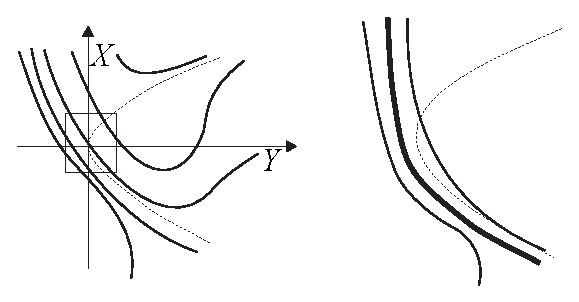
\includegraphics [scale=1.4]{jtr47}
	\caption{The phenomenon of `spurt'.}
	\label{fig:4.7}
\end{figure}

\subsubsection{B. Delay in the loss of stability.}
In this case, which corresponds to the Andronov-Hopf bifurcation, the problem is reduced to the following model system
\begin{equation}
\label{4.13}
\dot{z}=\left( y+i\omega \right) z+cz\left\vert z\right\vert ^{2},\text{ \ \
}\dot{y}=\varepsilon ,
\end{equation}
$z = x_{1}+ix_{2}\in \mathbb{C}\simeq \mathbb{R}^{2},$ $y\in \mathbb{R}.$ Of course, $y=\varepsilon t$ is a `flowing' parameter. Suppose further that
$$
c=-1;
$$
the case of $c> 0$ is less interesting. For the amplitude $r=\left\vert z\right\vert$ we get the Bernoulli equation
$$
\dot{r}=r\left( \varepsilon t-r^{2}\right).
$$

Let's put the initial condition
$$
y(t_{0})=-\mu ,\text{ \ \ \ }r(t_{0})=r_{0},\text{ \ \ }t_{0}=-\mu
/\varepsilon ,
$$
where $\mu >0$ is a fixed constant (not too big and not too small). This initial problem has the following solution
\begin{equation}
\label{4.14}
r(t)=r_{0}\left\{ e^{\varepsilon \left( t_{0}^{2}-t^{2}\right)
}+2r_{0}^{2}\int_{t_{0}}^{t}e^{\varepsilon \left( s^{2}-t^{2}\right)
}ds\right\} ^{-1/2}
\end{equation}
(Task 4.24). We will examine the asymptotic behavior of this solution at $\varepsilon \to 0$ by dividing the time range $t$ into four areas:
\begin{enumerate}[(a)]
	\item $0<t-t_{0}<O(1)$, or $0<y+\mu <O(\varepsilon ).$\\
	Let $u=t-t_{0}$. Then $\varepsilon \left( t_{0}^{2}-t^{2}\right)
	=\varepsilon (t_{0}+t)u\approx 2\mu u$ and $\varepsilon \left(
	s^{2}-t^{2}\right) \approx 2\mu (u-v)$, where $v=s-t_{0}$. Thus,
	$$
	\int_{t_{0}}^{t}e^{\varepsilon \left( s^{2}-t^{2}\right) }ds\approx
	\int_{0}^{u}e^{2\mu (u-v)}dv=\frac{1}{2\mu }(e^{2\mu u}-1)
	$$
	and
	$$
	r(t)\approx r_{0}\left\{ e^{2\mu u}+r_{0}^{2}(e^{2\mu u}-1)/\mu \right\}
	^{-1/2}
	$$
	is a decreasing function from $u$.
	\item $y=\varepsilon t$ is the set such that $-\mu <y<\mu$.\\
	Here, $e^{\varepsilon \left( t_{0}^{2}-t^{2}\right) }\approx e^{\left( \mu
		^{2}-y^{2}\right) /\varepsilon }\rightarrow \infty$. Thus,
	$$
	r(t)<C_{1}e^{-C_{2}/\varepsilon }\rightarrow 0,
	$$%
	which is a very quick pursuit of zero.
	\item $0<\left\vert t_{0}\right\vert -t<O(1)$, or $0<\mu -y<O(\varepsilon )$\\
	Let's introduce the variable $w=\left\vert t_{0}\right\vert -t$. As in case (a), we have $e^{\varepsilon \left( t_{0}^{2}-t^{2}\right) }\approx
	e^{2\mu w}.$
	
	We will divide the integration area for the integral in the formula \eqref{4.14} into three sections: from $t_{0}$ to $t_{0}/2<0$, from $t_{0}/2$ to $\left\vert t_{0}\right\vert /2$ and from $\left\vert t_{0}\right\vert /2$ to $t$. Through $I_{1},$ $I_{2}$ and $I_{3}$ we will determine the relevant integrals. Similarly as in case (a), it shows that $I_{1}=O(1)$ and $I_{3}=O(1)$. The calculations in (b) show that $I_{2}\to 0$ very quickly. Thus,
	$$
	r(t)=O(1).
	$$
	\item $\left\vert t_{0}\right\vert <t$, or $y>\mu $ and it is fixed. Now
	$e^{\left\{ \varepsilon \left( t_{0}^{2}-t^{2}\right) \right\}} \approx e^{\left\{ -(y^{2}-\mu ^{2})/\varepsilon \right\}} \to 0$. Then $\varepsilon \left( s^{2}-t^{2}\right) \approx (s-t)\cdot 2y$ for $s$ close to $t$, i.e. for those $s$, for which the contribution to the integral is dominant. We get $\int^{t}e^{2y(s-t)}ds \approx \frac{1}{2y}$. Hence
	$$
	r(t)\approx r_{0}\left\{ r_{0}^{2}/2y\right\} ^{-1/2}=\sqrt{y}.
	$$
\end{enumerate}

\begin{figure}[!ht]
	\centering
	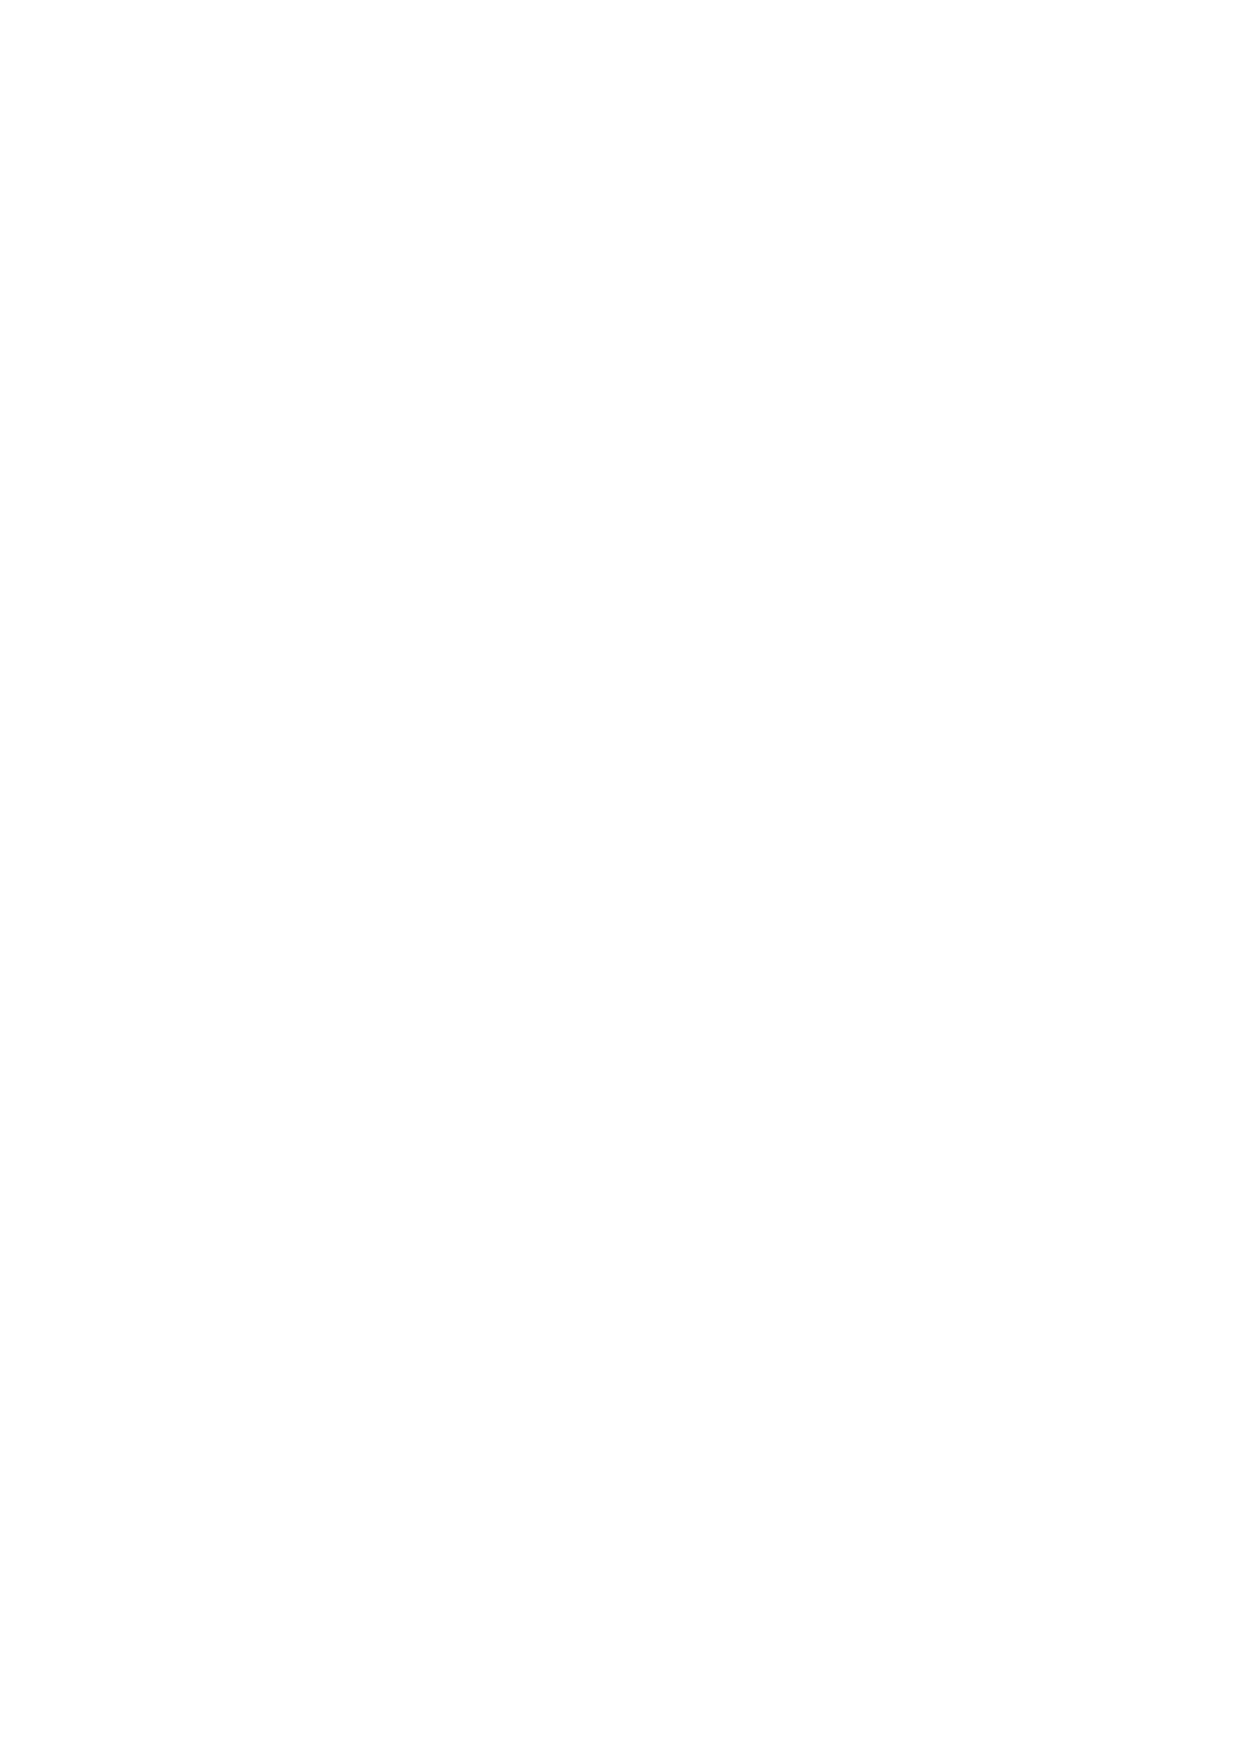
\includegraphics [scale=1.4]{jtr48}
	\caption{The phenomenon of delayed loss of stability.}
	\label{fig:4.8}
\end{figure}

We can summarize the above calculation.

\begin{theorem}
	In the case B described by the system \eqref{4.13} with $c <0$, the phenomenon of delay in the loss of stability occurs. It depends on changing the variable $y$ (which is the coefficient of unstable motion of stability) from the negative value $y(t_{0})=-\mu $ to the positive value $\mu $ the system (with respect to $z$) is stable all the time, and the change in the stability of the solution takes place for parameter $y = \mu $, whereby the amplitude of the oscillation increases as in the normal Andronov-Hopf bifurcation.
\end{theorem}

The phenomenon of \textbf{delay in the loss of stability} can be explained physically. The variable $y$ is negative for a very long time, on the order of $1/\varepsilon$. Then the physical system will come very close to the balance; close enough that you need the same amount of time later to leave the balance (see Figure \ref{fig:4.8}).


\subsection*{Tasks}
\begin{task}
	Prove formula \eqref{4.14}.
\end{task}
